\section{Establishing the Double Zeroes Property}
\label{Ch4:Sec:Double_Zeroes}

% At some point earlier on, maybe in Chapter 3, we need to stress that double zeroes means double zeroes in the radial sense, except double zeroes after composition with just the norm and not the norm squared. (We are using norm squared so that we can prove Schwartzness. Just the norm isn't enough because the norm isn't smooth.)

The way we prove that $a$ and $b$ have double zeroes at $E_8$ lattice points with norm $> \sqrt{2}$ (or at normalised $E_8$ lattice points with norm $> 1$) is by showing that $a\rad$ and $b\rad$ agree, for $r > 2$, with functions that have double zeroes at \textit{all} even integers. It will then follow that $a$ and $b$ have double zeroes at all points on the $E_8$ lattice with norm $> \sqrt{2}$, since all elements of $\Lambda_8$ have norm of the form $\sqrt{2n}$ for some $n \in \N$ (cf. \Cref{Ch2:Thm:E8_Properties}).

The strategy to prove these two equalities will be to perform a change of contours using a version of the Cauchy-Goursat Theorem and use the relations and transformation rules between the $\phi$- and $\psi$-functions to combine integrals so that the result is exactly $a\rad$ or $b\rad$.

The version of the Cauchy-Goursat Theorem we use is the following.

\begin{boxtheorem}[Cauchy-Goursat for Unbounded Contours]\label{Ch4:Thm:CauchyGoursat_Unbounded}
    Suppose $f : \C \to \C$ is a function such that $f(z) \to 0$ as $\Im(z) \to \infty$. Then, for all $x_1, y_1, x_2, y_2 \in \R$, if $f$ is holomorphic at $z$ for all $z \in \C$ with $x_1 < \Re(z) < x_2$ and $y_2 < \Im(z)$, then
    \begin{align*}
        \int_{x_1 + iy_1}^{x_1 + i\infty} f(z) \, \diff{z}
        = \int_{x_1 + iy_1}^{x_1 + iy_2} f(z) \, \diff{z}
        + \int_{x_1 + iy_2}^{x_2 + iy_2} f(z) \, \diff{z}
        + \int_{x_2 + iy_2}^{x_2 + i\infty} f(z) \, \diff{z}
    \end{align*}
    provided that $f$ is integrable on the unbounded vertical contours.
\end{boxtheorem}

\begin{wrapfigure}[7]{r}{0.4\linewidth}
    \vspace{-0.7em}
    \centering
    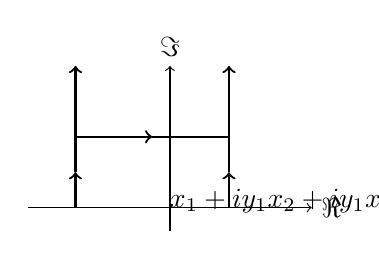
\begin{tikzpicture}[scale=1.5]
        % Axes
        \draw[->] (-1.2,0) -- (1.2,0) node[right] {$\Re$};
        \draw[->] (0,-0.2) -- (0,1.2) node[above] {$\Im$};
    
        % Contours
        \draw[thick, ->] (-0.8, 0) -- (-0.8,0.3);
        \draw[thick, ->] (-0.8,0.3) -- (-0.8, 1.2);
        \draw[thick, ->] (0.5, 0) -- (0.5,0.3);
        \draw[thick, ->] (0.5,0.3) -- (0.5, 1.2);
        \draw[thick, ->] (-0.8, 0.6) -- (-0.15, 0.6);
        \draw[thick] (-0.15, 0.6) -- (0.5, 0.6);
    
        % Points of interest
        \labelledpoint{-0.8}{0}{-0.4}{-0.8}{$x_1 + iy_1$}
        \labelledpoint{0.5}{0}{0.4}{-0.8}{$x_2 + iy_1$}
        \labelledpoint{-0.8}{0.6}{-0.8}{-0.3}{$x_1 + iy_2$}
        \labelledpoint{0.5}{0.6}{0.8}{-0.3}{$x_2 + iy_2$}
    \end{tikzpicture}
    \caption{Visualising the contours in \Cref{Ch4:Thm:CauchyGoursat_Unbounded}.}  
\end{wrapfigure}

We discuss the informal and formal proofs of this theorem in \Cref{Ch5:Sec:Cauchy-Goursat}.

For both $a\rad$ and $b\rad$, we begin by their alternate expressions for them. We then make estimates to prove that the integrals in these expressions converge. We finally manipulate the expressions and apply \Cref{Ch4:Thm:CauchyGoursat_Unbounded} to show that they do, indeed, agree with $a\rad$ and $b\rad$ on inputs $> 2$.

\subsection{The $+1$-Eigenfunction}

We begin by defining the integral by which we represent $a\rad$.

\begin{boxdefinition}[Alternate Representation of $a\rad$]
    Define $d : \parenth{2, \infty} \to \C$ by
    \begin{align*}
        d\of{r} = -4 \sinsq{\frac{\pi r}{2}} \int_{0}^{i\infty} \phi_0\of{\frac{-1}{z}} \, z^2 \, e^{\pi i r z} \, \diff{z}
    \end{align*}
    for all $r \in \parenth{2, \infty}$.
\end{boxdefinition}

It is clear that we can parametrise the integral in $d$ by $z = it$ for $t \in \parenth{0, \infty}$, and write
\begin{align}
    d(r) = 4i \sinsq{\frac{\pi r}{2}} \int_{0}^{\infty} \phi_0\of{\frac{i}{t}} \, t^2 \, e^{-\pi r t} \, \diff{t}
    \label{Ch4:Eq:d_parametrised}
\end{align}

We now show that this integral converges for $r > 2$. We do this by estimating the integrand.

\begin{boxlemma}
    $\exists C_0 > 0$ such that for $t \in \parenth{0, 2}$, $\abs{\phi_0\of{\frac{i}{t}}} \leq C_0 \, e^{-2\pi/t}$.
\end{boxlemma}
\begin{proof}
    This follows immediately from \eqref{Ch4:Eq:PolyFourierCoeffBound_phi_0}, with $z = i/t$.
\end{proof}

We can hence conclude that for $t \in \parenth{0, 2}$, the integrand in \eqref{Ch4:Eq:d_parametrised} is bounded:
\begin{align*}
    \abs{\phi_0\of{\frac{i}{t}} \, t^2 \, e^{-\pi r t}} 
    \leq 4 C_0 \, e^{-2\pi / t} \, e^{-\pi r t}
    \leq 4 C_0
\end{align*}

We can also estimate the integrand for $t \geq 2$.

\begin{boxlemma}\label{Ch4:Lemma:d_integral_estimate_above}
    $\exists C > 0$ such that for $t \geq 2$, $\abs{\phi_{0}\of{\frac{i}{t}}} \leq C t^{-2} e^{2\pi t}$.
\end{boxlemma}
\begin{proof}
    From \eqref{Ch4:Eq:phi_0_neg_inv}, we know that for all $t \geq 2$,
    \begin{align*}
        \abs{\phi_0\of{\frac{i}{t}}}
        = \abs{\phi_{0}\of{\frac{-1}{it}}}
        \leq \abs{\phi_{0\of{it}}} + \frac{12}{\pi t} \abs{\phi_{-2}\of{it}} + \frac{36}{\pi^2 t^2} \abs{\phi_{-4}\of{it}}
    \end{align*}
    Estimating each of these terms using \Cref{Ch4:Lemma:PolyFourierCoeffBound_Apply_a}, we know $\exists C_0, C_{-2}, C_{-4} > 0$ such that
    \begin{align*}
        \abs{\phi_{0}\of{it}} + \frac{12}{\pi t} \abs{\phi_{-2}\of{it}} + \frac{36}{\pi^2 t^2} \abs{\phi_{-4}\of{it}}
        \leq C_0 e^{-2 \pi t} + \frac{12}{\pi t} C_{-2} + \frac{36}{\pi^2 t^2} C_{-4} e^{2 \pi t}
    \end{align*}
    For $t \geq 2$, $C_0 e^{-2 \pi t}$ and $\frac{12}{\pi t} C_{-2}$ are clearly bounded by constants, and the growth of the above expression is dominated by $t^{-2} e^{2\pi t}$. Hence, we can conclude that $\exists C > 0$ such that for $t \geq 2$, $\abs{\phi_0\of{\frac{i}{t}}} \leq C t^{-2} e^{2 \pi t}$, as required.
\end{proof}

We can hence conclude that for $t \geq 2$, the integrand in \eqref{Ch4:Eq:d_parametrised} is bounded by an integrable function:
\begin{align*}
    \abs{\phi_0\of{\frac{i}{t}} \, t^2 \, e^{-\pi r t}} 
    \leq C \parenth{t^{-2} e^{2\pi t}} \parenth{t^2 e^{-\pi r t}}
    = C e^{\pi t \parenth{2 - r}}
\end{align*}
Here, we require $r > 2$ so that the exponent is negative. Since $d$ was defined precisely on such $r$, we can conclude that the integral in the definition of $d$ converges absolutely.

Arguing as above yields another important result.
\begin{boxlemma}\label{Ch4:Lemma:d_integrand_vanish_tendsto_ImInfty}
    For all $r > 2$ and $z \in \Halfplane$, as $\Im(z) \to \infty$,
    \begin{align*}
        \phi_{0}\of{\frac{-1}{z}} \, z^2 \, e^{\pi i r z} \to 0
    \end{align*}
\end{boxlemma}
% \begin{proof}[Proof sketch]
%     We do not offer more than a sketch here because the proof is almost identical to that of \Cref{Ch4:Lemma:d_integral_estimate_above}. The idea is to apply \eqref{Ch4:Eq:phi_0_neg_inv}, multiply through, apply \Cref{Ch4:Lemma:PolyFourierCoeffBound_Apply_a} to bound the expression in absolute value, and use the fact that $r > 2$ to conclude that the bound decays exponentially as $\Im(z) \to \infty$.
% \end{proof}

The function $z \mapsto \phi_{0}\of{\frac{-1}{z}} \, z^2 \, e^{\pi i r z}$ is also holomorphic on $\Halfplane$, a fact that is again seen by applying \eqref{Ch4:Eq:phi_0_neg_inv} and the fact that the numerators of the $\phi$-function are holomorphic and the denominators are non-vanishing on $\Halfplane$.

We are now ready for the main result of this subsection.

\begin{boxproposition}\label{Ch4:Prop:a_eq_d}
    For all $r > 2$, $d(r) = a\rad(r)$.
\end{boxproposition}
\begin{proof}
    Fix $r > 2$. Write $-4 \sinsq{\frac{\pi r}{2}} = e^{i \pi r} - 2 + e^{-i \pi r}$. Then, for all $r > 2$, we can write
    \begin{align} \small
         d(r)
         =
         \int_{0}^{i \infty} \phi_0\of{\frac{-1}{z}} z^2 e^{\pi i r \parenth{z - 1}} \diff{z}
         +
         \int_{1}^{1 + i \infty} \phi_0\of{\frac{-1}{z - 1}} \parenth{z - 1}^2 e^{\pi i r z} \diff{z}
         +
         \int_{0}^{i \infty} \phi_0\of{\frac{-1}{z}} z^2 e^{\pi i r \parenth{z + 1}} \diff{z}
         \label{Ch4:Eq:d_after_sinsq_trick}
    \end{align}
    Changing variables, we can express the integrals as follows.
    \begin{align*}
        \int_{0}^{i \infty} \phi_0\of{\frac{-1}{z}} z^2 \, e^{\pi i r \parenth{z - 1}} \, \diff{z}
        &=
        \int_{-1}^{-1 + i \infty} \phi_0\of{\frac{-1}{z + 1}} \parenth{z + 1}^2 \, e^{\pi i r z} \, \diff{z} \\
        \int_{0}^{i \infty} \phi_0\of{\frac{-1}{z}} z^2 \, e^{\pi i r \parenth{z + 1}} \, \diff{z}
        &=
        \int_{1}^{1 + i \infty} \phi_0\of{\frac{-1}{z - 1}} \parenth{z - 1}^2 \, e^{\pi i r z} \, \diff{z} \\
        -2 \int_{0}^{i \infty} \phi_0\of{\frac{-1}{z}} z^2 \, e^{\pi i r z} \, \diff{z}
        &=
        \underbrace{-2 \int_{0}^{i} \phi_0\of{\frac{-1}{z}} z^2 \, e^{\pi i r z} \, \diff{z}}_{I_5}
        -2 \int_{i}^{i \infty} \phi_0\of{\frac{-1}{z}} z^2 \, e^{\pi i r z} \, \diff{z} % \\
        % &= I_5(r) - 2\int_{i}^{i \infty} \phi_0\of{\frac{-1}{z}} z^2 \, e^{\pi i r z} \, \diff{z}
    \end{align*}
    We can now apply \Cref{Ch4:Thm:CauchyGoursat_Unbounded} to the first and third integrals, noting that the required integrability conditions do hold because the integrals making up $d$ and $a\rad$ converge absolutely.
    \begin{align*}
        \int_{-1}^{-1 + i \infty} \phi_0\of{\frac{-1}{z + 1}} \parenth{z + 1}^2 \, e^{\pi i r z} \, \diff{z}
        =& \underbrace{\int_{-1}^{-1 + i} \phi_0\of{\frac{-1}{z + 1}} \parenth{z + 1}^2 \, e^{\pi i r z} \, \diff{z}}_{I_1} \\
        &+ \underbrace{\int_{-1 + i}^{i} \phi_0\of{\frac{-1}{z + 1}} \parenth{z + 1}^2 \, e^{\pi i r z} \, \diff{z}}_{I_2} \\
        &+ \int_{i}^{i \infty} \phi_0\of{\frac{-1}{z + 1}} \parenth{z + 1}^2 \, e^{\pi i r z} \, \diff{z} \\
        % =& I_1(r) + I_2(r) + \int_{i}^{i \infty} \phi_0\of{\frac{-1}{z + 1}} \parenth{z + 1}^2 \, e^{\pi i r z} \, \diff{z} \\
        \int_{1}^{1 + i \infty} \phi_0\of{\frac{-1}{z - 1}} \parenth{z - 1}^2 \, e^{\pi i r z} \, \diff{z}
        =& \underbrace{\int_{1}^{1 + i} \phi_0\of{\frac{-1}{z - 1}} \parenth{z - 1}^2 \, e^{\pi i r z} \, \diff{z}}_{I_3} \\
        &+ \underbrace{\int_{1 + i}^{i} \phi_0\of{\frac{-1}{z - 1}} \parenth{z - 1}^2 \, e^{\pi i r z} \, \diff{z}}_{I_4} \\
        &+ \int_{i}^{i \infty} \phi_0\of{\frac{-1}{z - 1}} \parenth{z - 1}^2 \, e^{\pi i r z} \, \diff{z} % \\
        % =& I_3(r) + I_4(r) + \int_{i}^{i \infty} \phi_0\of{\frac{-1}{z - 1}} \parenth{z - 1}^2 \, e^{\pi i r z} \, \diff{z}
    \end{align*}
    Hence, we can express $d(r)$ as the sum of the following six integrals:
    \begin{align*}
        d(r) =& I_1(r) + I_2(r) + I_3(r) + I_4(r) + I_5(r) \\
        &+ \int_{i}^{i\infty} \parenth{
            \phi_0\of{\frac{-1}{z + 1}} \parenth{z + 1}^2 \, e^{\pi i r z} +
            \phi_0\of{\frac{-1}{z - 1}} \parenth{z - 1}^2 \, e^{\pi i r z} - 2
            \phi_0\of{\frac{-1}{z}} z^2 \, e^{\pi i r z}
        } \, \diff{z}
    \end{align*}
    One can show, by applying \eqref{Ch4:Eq:phi_0_neg_inv} and simplifying, that
    \begin{align*}
        \phi_0\of{\frac{-1}{z + 1}} \parenth{z + 1}^2 +
        \phi_0\of{\frac{-1}{z - 1}} \parenth{z - 1}^2 +
        \phi_0\of{\frac{-1}{z}} z^2 = 2\phi_0
    \end{align*}
    Hence, the sixth integral above is precisely $I_6$, proving that $d(r) = a\rad(r)$ for all $r > 2$.
\end{proof}

The factor of $-4\sinsq{\pi r / 2}$ in the definition of $d$ then ensures that $a\rad$ has double zeroes at all even integers except possibly $0$ and $\pm 2$, which allows us to conclude that $a$ has double zeroes at all points in $\R^8$---particularly those lying on $\Lambda_8$---with norm of the form $\sqrt{2n}$ for $n \in \N \setminus \set{0, 1}$.

\subsection{The $-1$-Eigenfunction}

We begin by defining the integral by which we represent $b\rad$.

\begin{boxdefinition}[Alternate Representation of $b\rad$]
    Define $c : \parenth{2, \infty} \to \C$ by
    \begin{align*}
        c\of{r} = -4 \sinsq{\frac{\pi r}{2}} \int_{0}^{i\infty} \psi_I\of{z} \, e^{\pi i r z} \, \diff{z}
    \end{align*}
    for all $r \in \parenth{2, \infty}$.
\end{boxdefinition}

It is clear that we can parametrise the integral in $d$ by $z = it$ for $t \in \parenth{0, \infty}$, and write
\begin{align}
    d(r) = 4i \sinsq{\frac{\pi r}{2}} \int_{0}^{\infty} \psi_T\of{it} \, e^{-\pi r t} \, \diff{t}
    \label{Ch4:Eq:c_parametrised}
\end{align}

We now show that this integral converges for $r > 2$. We do this by estimating the integrand.

\begin{boxlemma}
    $\exists C_S > 0$ such that for $t \in \parenth{0, 2}$, $\abs{\psi_I\of{it}} \leq C_S \, t^2 \, e^{\pi / t}$.
\end{boxlemma}
\begin{proof}
    From \eqref{Ch4:Eq:psi_I_to_psi_S}, we know that for all $t \in \parenth{0, 2}$,
    \begin{align*}
        \abs{\psi_I\of{it}}
        = \abs{\parenth{it}^2 \, \psi_S\of{\frac{-1}{it}}}
        = t^2 \abs{\psi_S\of{\frac{i}{t}}}
    \end{align*}
    Since $t < 2$, $\frac{1}{t} > \frac{1}{2}$. Hence, \Cref{Ch4:Lemma:PolyFourierCoeffBound_Apply_b} is applicable and yields exactly the desired result.
\end{proof}

Since $\parenth{0, 2}$ is clearly bounded, we can conclude that the integrand in \eqref{Ch4:Eq:c_parametrised} is bounded for $t \in \parenth{0, 2}$.

In similar fashion, we can estimate the integrand for $t \geq 2$.

\begin{boxlemma}
    $\exists C > 0$ such that for all $t \geq 2$, $\abs{\psi_I\of{it}} \leq C e^{2 \pi t}$.
\end{boxlemma}
\begin{proof}
    This follows immediately from \eqref{Ch4:Eq:PolyFourierCoeffBound_psi_I}, with $z = it$.
\end{proof}

We can hence conclude that for $t \geq 2$, the integrand in \eqref{Ch4:Eq:c_parametrised} is bounded by an integrable function:
\begin{align*}
    \abs{\psi_I\of{it} \, e^{- \pi r t}} \leq C \, e^{\pi t \parenth{2 - r}}
\end{align*}
where, as with $d$ in the previous subsection, we require $r > 2$ for the exponent $2 - r$ to be negative. We can hence conclude that $c$ converges absolutely. This gives us the integrability condition that is necessary to apply \Cref{Ch4:Thm:CauchyGoursat_Unbounded}. Indeed, this bound also tells us, as it did in \Cref{Ch4:Lemma:d_integrand_vanish_tendsto_ImInfty}, that
\begin{boxlemma}
    For all $r > 2$ and $z \in \Halfplane$, as $\Im(z) \to \infty$,
    \begin{align*}
        \psi_I\of{z} \, e^{\pi i r z} \to 0
    \end{align*}
\end{boxlemma}

We end our discussion on the integrand by remarking that it is holomorphic, as was discussed immediately after \Cref{Ch4:Prop:psi_as_div_disc}. We are now ready for the main result of this subsection.

\begin{boxproposition}\label{Ch4:Prop:b_eq_c}
    For all $r > 2$, $c(r) = b\rad(r)$.
\end{boxproposition}
\begin{proof}
    Fix $r > 2$. As in \eqref{Ch4:Eq:d_after_sinsq_trick}, we can write
    \begin{align*}
        c(r)
        = \int_{-1}^{-1 + i\infty} \psi_I\of{z + 1} e^{i\pi r z} \, \diff{z}
        - 2 \int_{0}^{i\infty} \psi_I\of{z} e^{i\pi r z} \, \diff{z}
        % - 2 \int_{i}^{i\infty} \psi_I\of{z} e^{i\pi r z} \, \diff{z}
        + \int_{1}^{1 + i\infty} \psi_I\of{z - 1} e^{i\pi r z} \, \diff{z}
    \end{align*}
    We may now apply \Cref{Ch4:Thm:CauchyGoursat_Unbounded} and write
    \begin{align*}
        \int_{-1}^{-1 + i\infty} \psi_I\of{z + 1} e^{i\pi r z} \, \diff{z}
        =& \int_{-1}^{-1 + i} \psi_I\of{z + 1} e^{i\pi r z} \, \diff{z} \\
        &+ \int_{-1 + i}^{i} \psi_I\of{z + 1} e^{i\pi r z} \, \diff{z} \\
        &+ \int_{i}^{i\infty} \psi_I\of{z + 1} e^{i\pi r z} \, \diff{z} \\
        \int_{1}^{1 + i\infty} \psi_I\of{z - 1} e^{i\pi r z} \, \diff{z}
        =& \int_{1}^{1 + i}\psi_I\of{z - 1} e^{i\pi r z} \, \diff{z} \\
        &+ \int_{1 + i}^{i} \psi_I\of{z - 1} e^{i\pi r z} \, \diff{z} \\
        &+ \int_{i}^{i\infty}\psi_I\of{z - 1} e^{i\pi r z} \, \diff{z}
    \end{align*}
    Applying \eqref{Ch4:Eq:psi_T_eq_psi_I_add_one} and \eqref{Ch4:Eq:psi_I_eq_psi_T_add_one} and splitting the integral from $0$ to $i\infty$ into two,
    \begin{align*}
        \int_{-1}^{-1 + i\infty} \psi_I\of{z + 1} e^{i\pi r z} \, \diff{z}
        &= J_1(r) + J_2(r) + \int_{i}^{i\infty} \psi_T\of{z} e^{i\pi r z} \, \diff{z} \\
        \int_{1}^{1 + i\infty} \psi_I\of{z - 1} e^{i\pi r z} \, \diff{z}
        &= J_3(r) + J_4(r) + \int_{i}^{i\infty} \psi_T\of{z} e^{i\pi r z} \, \diff{z} \\
        -2\int_{0}^{i\infty} \psi_I(z) e^{i \pi r z} &= J_5(r) - 2\int_{i}^{i\infty} \psi_I(z) e^{i \pi r z}
    \end{align*}
    \eqref{Ch4:Eq:psi_T_eq_psi_I_sub_psi_S} tells us that $\psi_S = \psi_T - \psi_I$. Hence,
    \begin{align*}
        c(r) = J_1(r) + J_2(r) + J_3(r) + J_4(r) + J_5(r) + J_6(r) = b\rad(r)
    \end{align*}
    for $r > 2$, as required.
\end{proof}

We can therefore conclude that $b$ has double zeroes at all points on $\Lambda_8$ with norm $> \sqrt{2}$.